\section{Foundations and Scope}
\label{sec:foundations}

\subsection{Introduction}
Physical AI concerns agents whose decisions change a physical environment. For a robot, choosing an action requires more than identifying a goal: the system must also contend with what is currently observable, how its body can move, and how objects may respond. A world model makes some of these consequences available as predictions. The central question for this survey is how such predictions contribute to learning and acting under the constraints of physical interaction.

Predictive models can support control through different computational routes. In \emph{World Models}, learned visual and temporal representations support policy learning, including training inside a learned environment~\cite{ha2018worldmodels}. PlaNet instead learns latent dynamics from images and uses online planning to select actions~\cite{hafner2019planet}. These examples motivate a distinction between using prediction to construct a policy and querying predictions while choosing an action. Their experimental settings establish particular uses of learned dynamics rather than a general guarantee of real-world competence.

Robot policies offer a complementary interface: they map observations and instructions to actions. OpenVLA, for example, adapts a vision-language backbone using robot demonstrations to produce visuomotor behavior~\cite{kim2024openvla}. This interface does not by itself expose a future-state predictor that can be queried under alternative actions. The distinction is functional: a policy may contain useful knowledge of dynamics, while an explicit prediction interface provides an additional object that can be inspected, optimized against, or compared with subsequent observations.

The relationship between representation learning and action-conditioned prediction also deserves separate treatment. V-JEPA~2 combines action-free video pretraining with a subsequent action-conditioned model, V-JEPA~2-AC, for robotic planning~\cite{assran2025vjepa2}. The stages serve different purposes and should not be assigned the same control interpretation solely because they share a representation. This motivates recording both the supervision that creates a representation and the interface through which a controller later uses it.

We organize the survey around three questions: \emph{what is predicted, how actions enter the model, and where prediction is used}. These are the survey's comparison axes. Together they connect data and model design to operational roles without requiring all systems to share one architecture or output space. A video generator, a latent predictor, and a structured dynamics model may address different parts of this design space; their comparison should identify the relevant state variables, time horizon, and control interface before assessing performance.

The same role-based approach guides evaluation. Evidence that a model predicts observations accurately supports a different claim from evidence that its predictions improve action selection. Likewise, a closed-loop task result must be interpreted with its task distribution, controller, inference budget, and failure conditions. Our synthesis therefore records predictive performance, downstream use, and deployment conditions separately. This is an analytical choice of the survey, not a universal ranking of papers or a requirement that every supporting component demonstrate a complete robot system.

The article follows four parts. Section~\ref{sec:foundations} establishes the scope and comparison axes. Section~\ref{sec:data} examines the data, representations, and modeling choices that determine which consequences can be learned. Section~\ref{sec:policy} studies how prediction interacts with policies, planning, memory, and recovery. Section~\ref{sec:evaluation} organizes evaluation, reliability, safety, and open problems around the claims that a deployed system must substantiate. A companion literature catalog retains the seven collection categories used by the project and links them to the writing process.

\subsection{Working Definitions and Inclusion Boundaries}
We use \emph{world model} for a learned model that predicts aspects of an environment's evolution from available information. For an action-conditioned world model, the inputs additionally specify actions or other interventions. The predicted variables may be observations, latent states, object relations, physical quantities, or task-relevant consequences. This working definition accommodates models learned from passive observations as well as interaction data; it does not assume that every predictive representation already provides an executable robot-action interface.

For analysis, let a history summarize the agent's observations and past actions. A policy maps this information and a goal to an action or action sequence. An action-conditioned world model maps the history and a proposed action sequence to predicted consequences. A controller turns the selected command into realized motion. Separating these interfaces lets us ask whether a failure originates in prediction, action selection, or execution, even when some interfaces are implemented inside a shared network.

The literature corpus includes both direct methods and supporting work. Learned simulators, predictive models used for planning, and prediction-guided policy learning provide direct cases. Datasets, analytical simulators, representation encoders, sensors, and policy baselines provide supporting context according to their demonstrated roles. Their inclusion does not imply that each item is itself a learned world model. In particular, the presence of a reasoning model in a control loop is insufficient to identify an explicit future-prediction mechanism.

\begin{figure}[t]
  \centering
  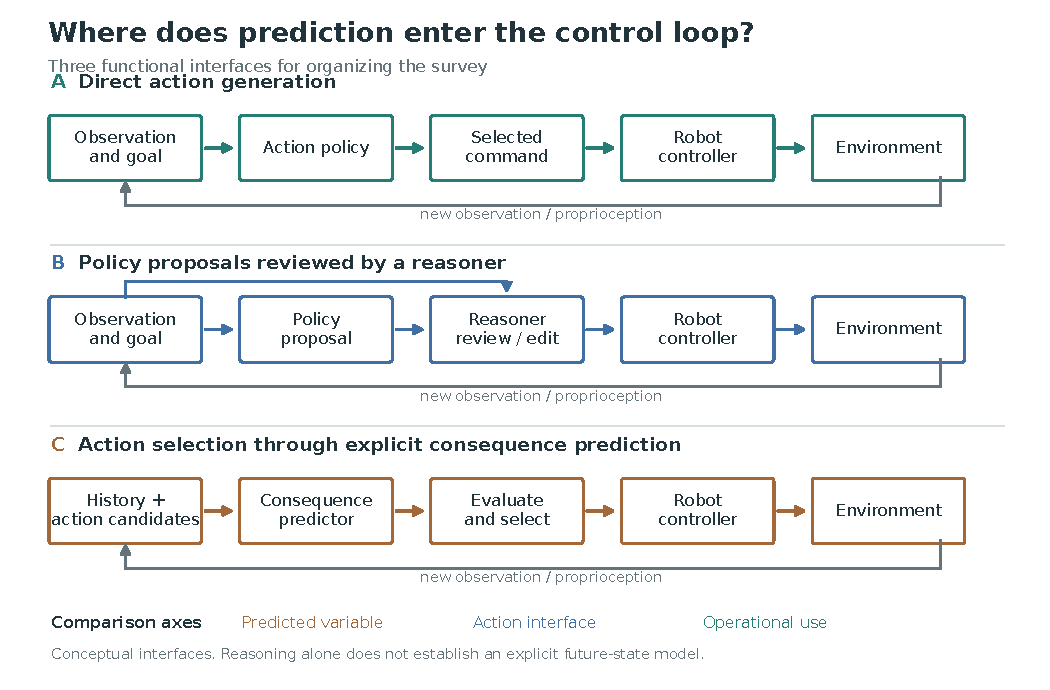
\includegraphics[width=\linewidth]{figures/fig01_prediction_policy_interfaces.pdf}
  \caption{Interfaces linking observation to physical action. The schematic distinguishes direct action generation, policy proposals reviewed by a reasoning model, and candidate actions evaluated through an explicit consequence predictor. Arrows denote interface-level information flow, not the internal architecture of any one model. Observation feedback closes each loop.}
  \Description{Three horizontal control loops. The first maps observations through a policy and controller to the environment. The second inserts a reasoner that reviews policy proposals and also receives observations. The third predicts consequences of action candidates before evaluation, selection, and control. Each loop returns new observations from the environment.}
  \label{fig:interfaces}
\end{figure}
